\documentclass[11pt, a4paper]{article}

% Packages
\usepackage{enumerate}
\usepackage{amsmath, amsfonts, amssymb, amsrefs}
\usepackage{textcomp}
\usepackage{geometry}
\usepackage{graphicx}
\usepackage{pgfplots}
\usepackage{caption}
\usepackage{subcaption}
\usepackage{float}
\usepackage{hyperref}

% Configurations
\allowdisplaybreaks
\pgfplotsset{compat=1.18}
\geometry{
	left=1in, 		 
	right=1in, 
	top=0.5in, 
	bottom=0.5in
} 
\hypersetup{
	colorlinks=true,
	linkcolor=[RGB]{0,158,74},
	citecolor=[RGB]{0,158,183}
}

% ..............Numbering...............
% reset equation counter at each section
\let\oldsection\section
\renewcommand{\section}{%
	\setcounter{equation}{0}%
	\oldsection%
}
\renewcommand{\thesection}{\Roman{section}}	% Section numbering
\renewcommand{\thesubsection}{\thesection.{\roman{subsection}}}	% subsection numbering
\renewcommand{\theequation}{\arabic{section}.\arabic{equation}}	% equation numbering

% New Commands
\newcommand{\novspace}{\vspace*{0pt}}
\newcommand{\nolinefrac}[2]{\genfrac{}{}{0pt}{}{#1}{#2}}
\newcommand{\numerator}[1]{\genfrac{}{}{0pt}{}{#1}{}}
\newcommand{\denominator}[1]{\genfrac{}{}{0pt}{}{}{#1}}
%\newcommand{\quotedsingle}[1]{\textquotesingle#1\textquotesingle}	% single quoted text
\newcommand{\quotedsingle}[1]{#1}	% quotes disabled
\newcommand{\quotedsingleit}[1]{\quotedsingle{\textit{#1}}}	% single quoted italic text
\newcommand{\eqrefnp}[1]{\textup{\ref{#1}}}  % Equation reference with no paranthesis

\newcommand{\primed}[1]{#1^{\prime}}
\newcommand{\tp}{\primed{t}}	% t prime
\newcommand{\omegap}{\primed{\omega}}	% omega prime
\newcommand{\xip}{\primed{\xi}}	% xi prime
\newcommand{\variance}[1]{\sigma_{#1}^{2}}
\newcommand{\stdev}[1]{\sigma_{#1}}

\newcommand{\diff}{\mathop{}\!\mathrm{d}}
\newcommand{\dx}{\diff x}
\newcommand{\dy}{\diff y}
\newcommand{\du}{\diff u}
\newcommand{\dt}{\diff t}
\newcommand{\dtp}{\diff \tp}
\newcommand{\domega}{\diff \omega}
\newcommand{\domegap}{\diff \omegap}
\newcommand{\dxi}{\diff \xi}
\newcommand{\dxip}{\diff \xip}

% Derivatives
\newcommand{\derv}[1]{\frac{\diff \hfill}{\diff #1}}	% Derivative without brackets
\newcommand{\dervb}[2]{\derv{#1} \left(#2\right)}  % Derivative with brackets
\newcommand{\dervsb}[2]{\derv{#1} \left[#2\right]}  % Derivative with square brackets
\newcommand{\dervf}[2]{\frac{\diff #2}{\diff #1 \hfil}}	% Derivative fractional form


% partial Differential signs
\newcommand{\pdiff}{\mathop{}\!\mathrm{\partial}} % Partial Differential sign
\newcommand{\pdx}{\pdiff x}
\newcommand{\pdy}{\pdiff y}
\newcommand{\pdt}{\pdiff t}
\newcommand{\pdtp}{\pdiff \tp}
\newcommand{\pdomega}{\pdiff \omega}
\newcommand{\pdomegap}{\pdiff \omegap}
\newcommand{\pdxi}{\pdiff \xi}
\newcommand{\pdxip}{\pdiff \xip}

% Partial Derivatives
\newcommand{\pderv}[1]{\frac{\pdiff \hfill}{\pdiff #1}}	% Partial Derivative without brackets
\newcommand{\pdervb}[2]{\pderv{#1} \left(#2\right)}  %Partial Derivative with brackets
\newcommand{\pdervsb}[2]{\pderv{#1} \left[#2\right]}  % Partial Derivative with square brackets


\newcommand{\dint}[2]{\int \limits_{#1}^{#2}}  % definite integral
\newcommand{\diint}[4]{\dint{#1}{#2} \dint{#3}{#4}}  % definite double integral
\newcommand{\diiint}[6]{\dint{#1}{#2} \dint{#3}{#4} \dint{#5}{#6}}  % definite triple integral
\newcommand{\intinfty}{\dint{-\infty}{\infty}}	% Integral from -infty to infty
\newcommand{\iintinfty}{\intinfty \intinfty}	% double Integral from -infty to infty
\newcommand{\iiintinfty}{\intinfty \intinfty \intinfty}	% triple Integral from -infty to infty
\newcommand{\intzerotoinfty}{\dint{0}{\infty}}	% integral from 0 to infty

% Global Info
\title{Fourier Transform: From Time to Space}
\author{Rohan Singh Chauhan}
\date{February 4, 2023}

% Main Document
\begin{document}
	\maketitle
	
	% Introduction
	\section{Introduction}\label{sec:intro}
	This paper focuses on an intuitive understanding of time, frequency and how they are related using Fourier Transform. Math behind such relationship is explored, which gives amazing insights that extends the corners of relativistic dynamics and quantum world. How this relationship manifests to a fundamental trade off that exists in nature, and how it is beautifully encapsulated in the language of mathematics is described in the text. Using principles of relativity and quantum mechanics, this idea is extended to space and all particles, and is then used to prove Quantum Uncertainty Principle, which shows how far fetching Fourier Transform can be...
	
	% The Fourier Transform
	\section{The Fourier Transform}\label{sec:fourier_transform}
	\subsection{Core Intuition}\label{sec:fourier_transform_intuition}
	The classical aim of Fourier Transform is frequency decomposition i.e given a signal, we want to find out what pure frequencies it is made up of. Concretely, it asks the question "How well a particular frequency correlates with the signal?". 
	
	Given some thought, this problem turns out to be similar to that of circular winding a mechanical spring. The physical analogy given here strikes to one's imagination. Consider for simplicity, a 2D linear spring made of metallic wire, which really is a projection of an actual 3D linear spring on a plane parallel to its axis. It is characterized by the number of turns per unit length along its axis without any applied load i.e \textbf{Free Turn Frequency} $\boldsymbol{f_{t}}$, which in this case is 2 turns/cm (figure \ref{fig:2d_linear_spring_turn_fq_2}). For argument sake, pretend that we don't know the turn frequency and our aim now is to construct a general way to find it out.
	
	If we take this 2D linear spring and wrap it around a circle centered at origin, essentially turning its axis circular, we will end up with a wound up circular spring which is now characterized by the number of times the linear axis of spring is coiled in circles (number of circular wraps) per unit length of its axis i.e \textbf{Wrapping Frequency} $\boldsymbol{f_{w}}$ (figure \ref{fig:wound_up_spring_plots}). The key idea here is that, though we cannot control free turn frequency of the spring, we can choose to wrap it around a circle less or more tightly, however we want i.e we have full control over the wrapping frequency. If we start with some low initial wrapping frequency and increase it over time, the weight of wound up spring turns out to centered near origin most of the time (fig \ref{fig:wound_up_spring_wrap_freq_min}, \ref{fig:wound_up_spring_wrap_freq_eq_turn_freq_by_4} and \ref{fig:wound_up_spring_wrap_freq_eq_turn_freq_by_2}). However, something very strange happens when wrapping frequency matches free turn frequency of the spring (like in most resonance phenomenon). In this case, weight of the spring is heavily off-centered from the origin (figure \ref{fig:wound_up_spring_wrap_freq_eq_turn_freq}).
	
	This observation can be expressed in terms of center of mass of the wound up spring, which is a 2D point on the reference plane. It is close to the origin for most of wrapping frequencies except when wrapping frequency is the same as free turn frequency, where it is significantly far from the origin. Plots of the center of mass for various winding frequencies are shown in figure \ref{fig:wound_up_spring_com_plots}. The spike at $f_{w} = 2$ wraps/cm means that it is the dominant turn frequency of spring. Hence, \textit{center of mass of the wound up spring is a measure of how well a wrapping frequency correlates with the linear spring turn frequency}. This idea forms the basis for general mathematical construct of frequency decomposition of signals.
	
	TODO: mathematical construct to find COM
	
	\begin{figure}
		\centering
		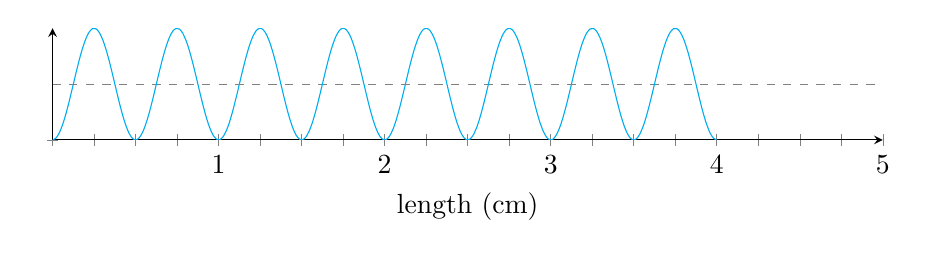
\begin{tikzpicture}
			\begin{axis} [
				axis lines=left, 
				xmin=0, 
				xmax=5, 
				ymin=0,
				ymax=2,
				xlabel=length (cm), 
				xtick distance=0.25,
				xticklabels={,,,,,1,,,,2,,,,3,,,,4,,,,5},
				ylabel=, 
				ylabel style={rotate=0}, 
				ytick=false,
				yticklabels={,,},
				width=\linewidth,
				height=3cm
				]
				
				\addplot[
				dashed,
				variable=\t,
				domain=0:5,
				color=gray, 
				mark=false
				] {
					1
				};
				
				\addplot[
				smooth,
				variable=\t,
				domain=0:4,
				color=cyan, 
				samples=200,
				mark=false
				] {
					cos((360 * 2 * t) + 180) + 1
				};
				
			\end{axis}
		\end{tikzpicture}
		
		\caption{A 2D linear spring with free length $4$ cm and free turn frequency $f_{t} = 2$ turns/cm. Dashed line represents spring axis.}
		\label{fig:2d_linear_spring_turn_fq_2}
	\end{figure}
	
	\begin{figure}
		\centering
		\subfloat[$f_{w} = f_{t}/8 = 0.25$ circular wraps/cm (or single wrap per $4$ cm free linear length of spring)] {
			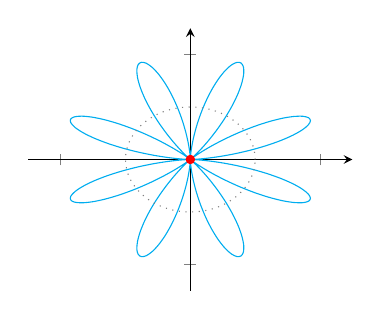
\begin{tikzpicture}
				\label{fig:wound_up_spring_wrap_freq_min}
				\begin{axis} [
					axis lines=middle, 
					xmin=-2.5, 
					xmax=2.5, 
					ymin=-2.5,
					ymax=2.5,
					xlabel=, 
					xticklabels={,,},
					ylabel=, 
					ylabel style={rotate=0}, 
					yticklabels={,,},
					width=0.47\linewidth
					]
					
					\addplot[
					smooth,
					variable=\t,
					domain=0:4,
					color=cyan, 
					samples=200,
					mark=false
					] (
					{ (cos((360 * 2 * t) + 180) + 1) * cos(360 * 0.25 * t) },
					{ (cos((360 * 2 * t) + 180) + 1) * sin(360 * 0.25 * t) }
					);
					
					\draw[dotted, color=gray, fill=none] (0, 0) circle (1.0);
					
					\draw[color=red, fill=red] (0,0) circle (1.5pt) node[above] {};
					
				\end{axis}
			\end{tikzpicture}
		}\hfill
		\subfloat[$f_{w} = f_{t}/4 = 0.5$ circular wraps/cm] {
			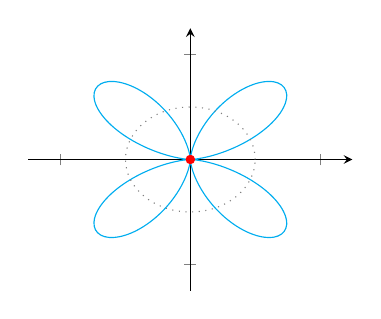
\begin{tikzpicture}
				\label{fig:wound_up_spring_wrap_freq_eq_turn_freq_by_4}
				\begin{axis} [
					axis lines=middle, 
					xmin=-2.5, 
					xmax=2.5, 
					ymin=-2.5,
					ymax=2.5,
					xlabel=, 
					xticklabels={,,},
					ylabel=, 
					ylabel style={rotate=0}, 
					yticklabels={,,},
					width=0.47\linewidth
					]
					
					\addplot[
					smooth,
					variable=\t,
					domain=0:4,
					color=cyan, 
					samples=200,
					mark=false
					] (
					{ (cos((360 * 2 * t) + 180) + 1) * cos(360 * 0.5 * t) },
					{ (cos((360 * 2 * t) + 180) + 1) * sin(360 * 0.5 * t) }
					);
					
					\draw[dotted, color=gray, fill=none] (0, 0) circle (1.0);
					
					\draw[color=red, fill=red] (0,0) circle (1.5pt) node[above] {};
					
				\end{axis}
			\end{tikzpicture}
		}
		
		\vspace{0.4cm}
		
		\subfloat[$f_{w} = f_{t}/2 = 1$ circular wrap/cm] {
			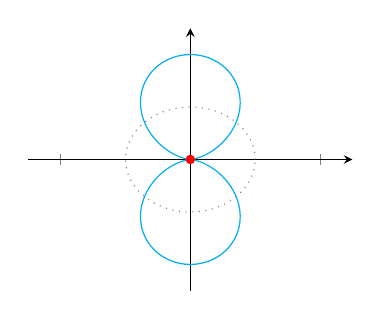
\begin{tikzpicture}
				\label{fig:wound_up_spring_wrap_freq_eq_turn_freq_by_2}
				\begin{axis} [
					axis lines=middle, 
					xmin=-2.5, 
					xmax=2.5, 
					ymin=-2.5,
					ymax=2.5,
					xlabel=, 
					xticklabels={,,},
					ylabel=, 
					ylabel style={rotate=0}, 
					yticklabels={,,},
					width=0.47\linewidth
					]
					
					\addplot[
					smooth,
					variable=\t,
					domain=0:4,
					color=cyan, 
					samples=200,
					mark=false
					] (
					{ (cos((360 * 2 * t) + 180) + 1) * cos(360 * 1 * t) },
					{ (cos((360 * 2 * t) + 180) + 1) * sin(360 * 1 * t) }
					);
					
					\draw[dotted, color=gray, fill=none] (0, 0) circle (1.0);
					
					\draw[color=red, fill=red] (0,0) circle (1.5pt) node[above] {};
					
				\end{axis}
			\end{tikzpicture}
		}\hfill
		\subfloat[$f_{w} = f_{t} = 2$ circular wraps/cm] {
			\begin{tikzpicture}
				\label{fig:wound_up_spring_wrap_freq_eq_turn_freq}
				\begin{axis} [
					axis lines=middle, 
					xmin=-2.5, 
					xmax=2.5, 
					ymin=-2.5,
					ymax=2.5,
					xlabel=, 
					xticklabels={,,},
					ylabel=, 
					ylabel style={rotate=0}, 
					yticklabels={,,},
					width=0.47\linewidth
					]
					
					\addplot[
					smooth,
					variable=\t,
					domain=0:4,
					color=cyan, 
					samples=200,
					mark=false
					] (
					{ (cos((360 * 2 * t) + 180) + 1) * cos(360 * 2 * t) },
					{ (cos((360 * 2 * t) + 180) + 1) * sin(360 * 2 * t) }
					);
					
					\draw[dotted, color=gray, fill=none] (0, 0) circle (1.0);
					
					\draw[color=red, fill=red] (-0.5,0) circle (1.5pt) node[above] {};
					
				\end{axis}
			\end{tikzpicture}
		}
		
		\caption{2D linear spring with free turn frequency $f_{t} = 2$ turns/cm wrapped around a circle centered at origin with various wrapping frequencies $f_{w}$. Red dot represents center of mass (COM) and the dotted circle represents axis of the wound up spring}
		\label{fig:wound_up_spring_plots}
	\end{figure}
	
	\begin{figure}
		\centering
		\subfloat[x-coordinate of COM vs $f_{w}$] {
			\begin{tikzpicture}
				\label{fig:wound_up_spring_com_xcoord_vs_wrap_freq}
				\begin{axis} [
					axis lines=left, 
					xmin=0, 
					xmax=4, 
					ymin=-0.5,
					ymax=2.5,
					xlabel=$f_{w}$, 
					ylabel=x-coordinate of COM, 
					ylabel style={rotate=0}, 
					width=0.47\linewidth
					]
					
					\addplot[thin, smooth, color=red] table [header=false, col sep=comma, x index=0, y index=1] {res/data/wound_up_spring_com_real.csv};
					
				\end{axis}
			\end{tikzpicture}
		}\hfill
		\subfloat[Distance of COM from origin vs $f_{w}$] {
			\begin{tikzpicture}
				\label{fig:wound_up_spring_com_distance_vs_wrap_freq}
				\begin{axis} [
					axis lines=left, 
					xmin=0, 
					xmax=4, 
					ymin=0,
					ymax=2.5,
					xlabel=$f_{w}$, 
					ylabel=distance of COM, 
					ylabel style={rotate=0}, 
					width=0.47\linewidth
					]
					
					\addplot[thin, smooth, color=red] table [header=false, col sep=comma, x index=0, y index=1] {res/data/wound_up_spring_com_magnitude.csv};
					
				\end{axis}
			\end{tikzpicture}
		}
		
		\caption{Center of mass (COM) of the wound up spring for various wrapping frequencies $f_{w}$}
		\label{fig:wound_up_spring_com_plots}
	\end{figure}
	
	
	\subsection{Definition}\label{sec:fourier_transform_def}  % Formal Definition
	Fourier transform of a complex valued function in time $f(t)$ (a signal) is another complex valued function in frequency $\hat{F}(\omega)$ (i.e spectrum), whose output for a certain frequency encodes the strength ($=absolute(\hat{F}(\omega))$) and phase offset ($=argument(\hat{F}(\omega))$) of that frequency within the original signal \cite{herman2016fourieranalysis}
	\begin{equation}\label{eq:ft_def}
		\boxed{
			\hat{F}(\omega) = \intinfty f(t)e^{-i\omega t} \dt
		}
	\end{equation}
	In general, if y is in reciprocal space of x, then
	\begin{equation*}\label{eq:ft_def_general}
		\hat{F}(y) = \intinfty f(x)e^{-ixy} \dx
	\end{equation*}
	So if x is time in seconds, then y represents temporal frequency in $s^{-1}$ (or $Hz$). Similarly if x is distance in meters, then y symbolizes spatial frequency in $m^{-1}$.
	
	\subsection{Rise of uncertainty}\label{sec:fourier_transform_intuitive_uncertainty}
	TODO: How uncertainty arises
	
	% Inverse Fourier Transform
	\section{Inverse Fourier Transform}\label{sec:inverse_fourier_transform}
	Given the Fourier transform $\hat{F}(\omega)$ of a function $f(t)$, the original function can be synthesized using
	
	\begin{equation}\label{eq:inverse_ft_def}
		\boxed{
			f(t) = \frac{1}{2\pi} \intinfty \hat{F}(\omega)e^{i\omega t} \domega
		} \qquad \text{if $\hat{F}(\omega)$ is integrable}
	\end{equation}
	This is known as \textbf{Fourier Inversion Theorem}, which allows a signal to be reconstructed from it's frequency and phase information. \cite{herman2016fourieranalysis}
	
	\vspace{4pt}
	\textbf{Proof}: \textit{(uses Appendix \ref{sec:fubini_theorem} and \ref{sec:delta_func})} Multiplying both sides of equation \eqref{eq:ft_def} with $e^{i\omega \tp}$ (note $\tp$ in place of $t$) and integrating with respect to $\omega$ gives
	\begin{align*}
		\intinfty e^{i\omega \tp} \hat{F}(\omega) \domega 
		= & \intinfty e^{i\omega \tp} \left(\intinfty f(t) e^{-i\omega t} \dt \right) \domega \\
		= & \iintinfty f(t) e^{-i\omega (t - \tp)} \dt \domega
		= \intinfty f(t) \left(\intinfty  e^{-i\omega (t - \tp)} \domega \right) \dt \tag{using \eqrefnp{eq:fubini}} \\
		= & \, 2 \pi \intinfty f(t) \delta (\tp - t) \dt = \, 2 \pi f(\tp) \tag{using \eqrefnp{eq:delta_func_def_complex_exp} and \eqrefnp{eq:delta_func_integration_value}}
	\end{align*} 
	replacing $\tp$ by $t$ gives the final form as in equation \eqref{eq:inverse_ft_def}
	
	% Michel Plancherel's (1885-1967) Theorem (or Parseval's identity for fourier Transform)
	\section{Plancherel's Theorem}\label{sec:plancherel_theorem}
	Fourier transform version of \quotedsingleit{Parseval's identity for Fourier Series}, given by Michel Plancherel (1885-1967) in 1910, called the Plancherel's Theorem is \cite{herman2016fourieranalysis}
	
	\begin{equation}\label{eq:plancherel_theorem}
		\intinfty |f(t)|^{2} \dt = \frac{1}{2 \pi} \intinfty |\hat{F}(\omega)|^{2} \domega
	\end{equation}
	which means that area under the square modulus of a function $|f(t)|^{2}$ is equal to area under the square modulus of it's spectrum $|\hat{F}(\omega)|^{2}$
	
	\vspace{4pt}
	\noindent
	\textbf{Proof}: 
	%using Fourier inversion theorem \eqref{eq:inverse_ft_def} and Fubini's theorem \eqref{eq:fubini}
	\begin{align*}
		\intinfty |f(t)|^{2} \dt 
		= & \intinfty f(t)f^{\star}(t) \dt \\
		= & \intinfty \left(\frac{1}{2 \pi} \intinfty \hat{F}(\omega) e^{i \omega t} \domega \right) \left(\frac{1}{2 \pi} \intinfty \hat{F}^{\star}(\omegap) e^{-i \omegap t} \domegap \right) \dt \tag{using \eqrefnp{eq:inverse_ft_def}} \\
		= & \frac{1}{(2 \pi)^2} \iiintinfty \hat{F}(\omega) \hat{F}^{\star}(\omegap) e^{i (\omega - \omegap) t} \domega \domegap \dt \\
		= & \frac{1}{(2 \pi)^2} \iintinfty \hat{F}(\omega) \hat{F}^{\star}(\omegap) \left( \intinfty e^{i (\omega - \omegap) t} \dt \right) \domega \domegap \tag{using \eqrefnp{eq:fubini}} \\
		= & \frac{1}{2 \pi} \iintinfty \hat{F}(\omega) \hat{F}^{\star}(\omegap) \delta(\omega - \omegap) \domega \domegap \tag{using \eqrefnp{eq:delta_func_def_complex_exp}} \\
		= & \frac{1}{2 \pi} \intinfty \hat{F}(\omega) \hat{F}^{\star}(\omega) \domega 
		= \frac{1}{2 \pi} \intinfty |\hat{F}(\omega)|^{2} \domega  \tag{using \eqrefnp{eq:delta_func_integration_value}} \\
	\end{align*}
	\noindent
	\textbf{Special Case}: If $f(t)$ is a probability distribution, then $|f(t)|^{2}$ represents the probability of occurrence of t (like a wave function). In that case, $\hat{F}(\omega)$ will also be a probability distribution. If $f(t)$ is normalized, \eqref{eq:plancherel_theorem} gives
	\begin{equation}\label{eq:plancherel_normal_func_and_spectrum}
		\intinfty |f(t)|^{2} \dt = 1 \qquad \text{and} \qquad \intinfty |\hat{F}(\omega)|^{2} \domega = 2 \pi
	\end{equation}
	
	% Fourier Uncertainty Principle
	\section{Fourier Uncertainty Principle}\label{sec:fourier_uncertainity_principle}
	A signal $f(t)$ and it's frequency representation $\hat{F}(\omega)$ are closely related. If a signal is localized (made out of observation over a short period of time), then it correlates well with wide range of frequencies i.e it's spectrum is spread out. It gets really ambiguous as to what frequencies it is actually made up of.
	
	However, observation over long period of time gives a spread out signal, which correlates only with certain frequencies, resulting in a concentrated spectrum. This makes the detection of constituent frequencies clear.
	
	This gives rise to a \quotedsingleit{\textbf{Natural Trade Off}} as to how concentrated a signal and it's frequency representation can be. It is illustrated more mathematically in following sections.
	
	\subsection{Qualitative: The Fourier Trade Off}\label{sec:fourier_uncertainity_principle_qualitative}
	let $f(t)$ be a continuous and integrable function over $\mathbb{R}$, and $g(t) = \frac{1}{\sqrt{k}} f \left( \frac{t}{k} \right)$ be a wrapper over $f(t)$, where $k$ is \quotedsingleit{spread constant} since it controls the spread of $g(t)$ (see figure \ref{fig:fourier_tradeoff_signal}) \cite{dubey2021fourieruncertainity}
	\begin{align*}
		\hat{G}(\omega) = & \intinfty g(t) e^{-i \omega t} \dt
		= \intinfty \left[ \frac{1}{\sqrt{k}} f \left( \frac{t}{k} \right) \right] e^{-i \omega t} \dt  \tag{using \eqrefnp{eq:ft_def}} \\
		= & \frac{1}{\sqrt{k}} \intinfty f(u) e^{-i \omega (uk)} \, k \du  \tag{where $u = \frac{t}{k}$} 
		= \sqrt{k} \intinfty f(u) e^{-i (k \omega) u} \du = \sqrt{k} \hat{F}(k \omega) 
	\end{align*}
	\begin{equation}\label{eq:fourier_tradeoff_spectrum}
		\boxed{
			\hat{G}(\omega) = \sqrt{k} \hat{F}(k \omega)
		}
	\end{equation}
	
	As $k$ increases, $g(t)$ spreads out, but it's spectrum $\hat{G}(\omega)$ gets localized (from eq \eqrefnp{eq:fourier_tradeoff_spectrum}). On the flip side, as $k$ decreases, $g(t)$ localizes and $\hat{G}(\omega)$ spreads out. In either case, one of them is localized (certain) and other is inevitably spread (uncertain) (see figure \ref{fig:fourier_tradeoff}). This is known as the \textbf{\textit{Fourier Trade Off}}
	
	\begin{figure}[H]
		\centering
		\subfloat[$g(t)$ vs $t$] {
			\label{fig:fourier_tradeoff_signal}
			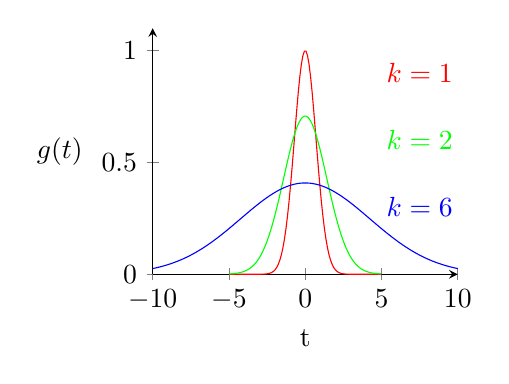
\begin{tikzpicture}
				\begin{axis} [
					axis lines=left, 
					xmin=-10, 
					xmax=10, 
					ymax=1.1,
					xlabel=t, 
					ylabel=$g(t)$, 
					ylabel style={rotate=-90}, 
					width=0.45\linewidth
					]
					
					\addplot[
					color=red, 
					samples=100,
					mark=false
					] {
						exp(-x^2)
					};
					
					\addplot[
					color=green, 
					samples=100, 
					mark=false
					] {
						(1 / sqrt(2)) * exp(-(x/2)^2)
					};
					
					\addplot[
					color=blue, 
					samples=100, 
					mark=false, 
					domain=-10:10
					] {
						(1 / sqrt(6)) * exp(-(x/6)^2)
					};
					
					\node at (axis cs:7.5,0.9){\color{red}$k=1$};
					\node at (axis cs:7.5,0.6){\color{green}$k=2$};
					\node at (axis cs:7.5,0.3){\color{blue}$k=6$};
				\end{axis}
			\end{tikzpicture}
		}\hfill
		\subfloat[$\hat{G}(\omega)$ vs $\omega$] {
			\label{fig:fourier_tradeoff_spectrum}
			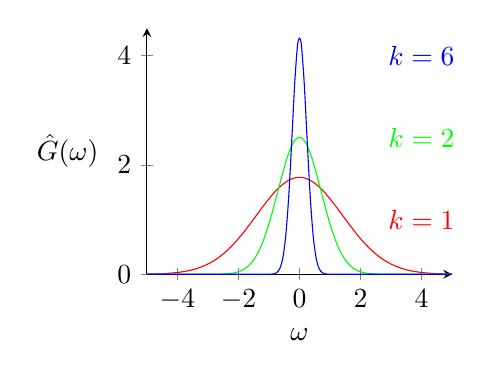
\begin{tikzpicture}
				\begin{axis}[
					axis lines=left, 
					xmin=-5,
					xmax=5,
					ymax=4.5,
					xlabel=$\omega$, 
					ylabel=$\hat{G}(\omega)$, 
					ylabel style={rotate=-90}, 
					width=0.45\linewidth
					]
					
					\addplot[
					smooth,
					samples=100, 
					color=red, 
					mark=false
					] {
						sqrt(pi) * exp(-(x^2) / 4)
					};
					
					\addplot[
					smooth,
					samples=100,
					color=green, 
					mark=false
					] {
						sqrt(2 * pi) * exp(-((2 * x)^2) / 4)
					};
					
					\addplot[
					smooth,
					samples=100, 
					color=blue, 
					mark=false
					] {
						sqrt(6 * pi) * exp(-((6 * x)^2) / 4)
					};
					
					\node at (axis cs:4,1.0){\color{red}$k=1$};
					\node at (axis cs:4,2.5){\color{green}$k=2$};
					\node at (axis cs:4,4.0){\color{blue}$k=6$};
				\end{axis}
			\end{tikzpicture}
		}
		
		%	\caption{signals $g(t)=\frac{1}{\sqrt{k}} f \left( \frac{t}{k} \right)$ where $f(t) = e^{-x^2}$ (Gaussian) and their corresponding spectrum $\hat{G}(\omega) = \sqrt{k} \hat{F}(k \omega)$ where $\hat{F}(\omega) = \sqrt{\pi} e^{\frac{-\omega^2}{4}}$ (another Gaussian) for different values of \textit{spread constant} $k$}
		
		\caption{An illustration of \textit{Fourier Trade Off} for a Gaussian $f(t) = e^{-t^2}$ and $\hat{F}(\omega) = \sqrt{\pi} e^{-\frac{\omega^2}{4}}$. Wrapper $g(t)=\frac{1}{\sqrt{k}} f \left( \frac{t}{k} \right)$, $\hat{G}(\omega) = \sqrt{k} \hat{F}(k \omega)$, where $k$ is \textit{spread constant}}
		
		\label{fig:fourier_tradeoff}  % Must label after caption
	\end{figure}
	
	\subsection{Quantitative: The Uncertainty Principle}
	The idea of fundamental trade off (section \ref{sec:fourier_uncertainity_principle_qualitative}) gives rise to a interesting question: \textit{Is there any quantitative aspect of this trade-off?}. More precisely: \textit{Is there any lower bound to the total uncertainty in time and frequency?}.
	
	This requires \quotedsingleit{uncertainty} to be defined, which is \textbf{probabilistic} and should not be confused with \textbf{possibility}. Latter is an absolute concept, where something being impossible eliminates it's existence entirely, while probability is a relative concept, where something being highly probable still retains the possibility of occurrence of low probable event.
	
	The key idea here is that $\boldsymbol{f(t)}$ \textbf{is a continuous probability distribution}, where $|f(t)|^{2}$ gives the probability (and not possibility) of occurrence of t. Likewise, it's spectrum $\hat{F}(\omega)$ is also a probability distribution.
	\begin{equation*}
		\text{Probability of occurrence of t: }P(t) = \frac{|f(t)|^{2}}{\intinfty |f(t)|^{2} \dt}
	\end{equation*}
	For a discrete random variable x, with probability $P(x)$, average $x = \bar{x} = \sum \limits_{i} x_{i} P(x_{i})$ and variance (spread of distribution about the mean) $ \variance{x} = \sum \limits_{i} (x_{i} - \bar{x})^{2} P(x_{i})$. Similarly
	
	% Definitions of mean and variance
	\begin{subequations}
		\begin{align}
			& \text{average } t = \bar{t} = \intinfty t P(t) \dt = \frac{\intinfty t |f(t)|^{2} \dt}{\intinfty |f(t)|^{2} \dt} \label{eq:avg_t} \\
			& \text{average } \omega = \bar{\omega} = \intinfty \omega P(\omega) \domega = \frac{\intinfty \omega |\hat{F}(\omega)|^{2} \domega}{\intinfty |\hat{F}(\omega)|^{2} \domega} \label{eq:avg_omega} \\
			& \text{variance in t} = \variance{t} = \intinfty (t - \bar{t})^{2} P(t) \dt = \frac{\intinfty (t - \bar{t})^{2} |f(t)|^{2} \dt}{\intinfty |f(t)|^{2} \dt} \label{eq:variance_t} \\
			& \text{variance in $\omega$} = \variance{\omega} = \intinfty (\omega - \bar{\omega})^{2} P(\omega) \domega = \frac{\intinfty (\omega - \bar{\omega})^{2} |\hat{F}(\omega)|^{2} \domega}{\intinfty |\hat{F}(\omega)|^{2} \domega} \label{eq:variance_omega}
		\end{align}
	\end{subequations}
	
	In the context of distributions, \textit{\textbf{Uncertainty} means the extent of spread of a distribution about it's mean value}, which is represented by standard deviation $\stdev{t}$ about the mean. Intuitively, high uncertainty means that if the measurement is repeated, their is a high chance of getting a value other than mean, giving a spread out probability distribution (and vice-versa).
	
	\vspace{4pt}
	Our goal is to find a lower bound to the total uncertainty (or spread) in $t$ (signal) and $\omega$ (spectrum), if that even exist. Mathematically, $\stdev{t}\, \stdev{\omega} \geq \, ?$. For simplicity, let $f(t)$ be a continuous, normalized probability distribution centered at $t=0$
	%$\bar{t}=0$, $\intinfty |f(t)|^{2} \dt = 1$ and  $\intinfty |\hat{F}(\omega)|^{2} \domega = 2\pi$ (using \eqref{eq:plancherel_normal_spectrum}) 
	% Assumptions
	\begin{subequations}
		\begin{align}
			& avg(t) = \bar{t} = 0 \qquad \text{(centered at $t = 0$)} \label{eq:assump_avg_t_0} \\
			& \intinfty |f(t)|^{2} \dt = 1 \qquad \text{and} \qquad \intinfty |\hat{F}(\omega)|^{2} \domega = 2\pi \qquad \text{(using \eqrefnp{eq:plancherel_normal_func_and_spectrum})} \label{eq:assump_normal_func_and_spectrum} \\
			& \variance{\omega} = \frac{1}{2\pi} \intinfty (\omega - \bar{\omega})^{2} |\hat{F}(\omega)|^{2} \domega  \qquad \text{(using \eqrefnp{eq:variance_omega} and \eqrefnp{eq:assump_normal_func_and_spectrum})} \label{eq:assump_variance_omega}
		\end{align}
	\end{subequations}
	Defining a function (which at first looks random, but have the ability to relate $\stdev{t}$ with $\stdev{\omega}$)\cite{dubey2021fourieruncertainity}
	\begin{equation}\label{eq:uncertainity_main_functionl}
		h_{k}(\omega) = \frac{(\omega - \bar{\omega})}{k \variance{\omega}} \hat{F}(\omega) + \derv{\omega}\hat{F}(\omega) \qquad \text{ where } k \in \mathbb{R} \text{ and } k \neq 0
	\end{equation}
	and the integral 
	\begin{equation}\label{eq:uncertainity_main_integral}
		I(k) = \intinfty |h_{k}(\omega)|^2 \domega
	\end{equation}
	The key idea here is that $I(k)$ is an integral of square modulus, hence $I(k) \geq 0$
	\begin{equation}\label{eq:uncertainity_main_integral_geq_0}
		I(k) = \intinfty |h_{k}(\omega)|^2 \domega = \intinfty h_{k}(\omega) \, h_{k}^{\star}(\omega) \domega \geq 0
	\end{equation}
	%\begin{align*}
	%	I(k) & = \intinfty \left[\frac{(\omega - \bar{\omega})}{k \variance{\omega}} \hat{F}(\omega) + \derv{\omega}\hat{F}(\omega)\right] \left[\frac{(\omega - \bar{\omega})}{k \variance{\omega}} \hat{F}^{\star}(\omega) + \derv{\omega}\hat{F}^{\star}(\omega)\right] \domega \tag{using \eqrefnp{eq:uncertainity_main_functionl}} \\
	%	& = \intinfty \left[\frac{(\omega - \bar{\omega})^{2}}{k^{2} \stdev{\omega}^{4}} |\hat{F}(\omega)|^{2} + \frac{(\omega - \bar{\omega})}{k \variance{\omega}}\left(\hat{F}(\omega) \dervf{\omega}{\hat{F}^{\star}}\numerator{(\omega)} + \hat{F}^{\star}(\omega) \dervf{\omega}{\hat{F}}\numerator{(\omega)} \right) + \dervf{\omega}{\hat{F}}\numerator{(\omega)} \dervf{\omega}{\hat{F}^{\star}}\numerator{(\omega)}
	%	\right] \domega
	%\end{align*}
	\begin{align*}
		I(k) & = \intinfty \left[\frac{(\omega - \bar{\omega})}{k \variance{\omega}} \hat{F}(\omega) + \derv{\omega}\hat{F}(\omega)\right] \left[\frac{(\omega - \bar{\omega})}{k \variance{\omega}} \hat{F}^{\star}(\omega) + \derv{\omega}\hat{F}^{\star}(\omega)\right] \domega \tag{using \eqrefnp{eq:uncertainity_main_functionl}} \\
		& = \intinfty \left[\frac{(\omega - \bar{\omega})^{2}}{k^{2} \stdev{\omega}^{4}} |\hat{F}(\omega)|^{2} + \frac{(\omega - \bar{\omega})}{k \variance{\omega}}\left(\hat{F}(\omega) \dervf{\omega}{\hat{F}^{\star}} + \hat{F}^{\star}(\omega) \dervf{\omega}{\hat{F}} \right) + \dervf{\omega}{\hat{F}} \dervf{\omega}{\hat{F}^{\star}}
		\right] \domega \\
		& = \intinfty \left[\frac{(\omega - \bar{\omega})^{2}}{k^{2} \stdev{\omega}^{4}} |\hat{F}(\omega)|^{2} + \frac{(\omega - \bar{\omega})}{k \variance{\omega}}\dervb{\omega}{\hat{F}(\omega) \hat{F}^{\star}(\omega)} + \dervf{\omega}{\hat{F}}\numerator{(\omega)} \dervf{\omega}{\hat{F}^{\star}\numerator{(\omega)}}
		\right] \domega
	\end{align*}
	\begin{equation}\label{eq:uncertainty_integral_triplet}
		\text{Hence,} \qquad I(k) = I_{1}(k) + I_{2}(k) + I_{3}
	\end{equation}
	Computing these terms separately, first term is
	\begin{equation}\label{eq:uncertainty_integral_part1}
		I_{1}(k) = \frac{1}{k^{2} \stdev{\omega}^{4}} \intinfty (\omega - \bar{\omega})^{2} |\hat{F}(\omega)|^{2} \domega = \frac{2 \pi \variance{\omega}}{k^{2} \stdev{\omega}^{4}} = \frac{2\pi}{k^{2} \variance{\omega}} \qquad \text{(using \eqrefnp{eq:assump_variance_omega})}
	\end{equation}
	Second term contains derivative and can be integrated by parts 
	%\frac{(\omega - \bar{\omega})}{k \variance{\omega}}\dervb{\omega}{\hat{F}(\omega) \hat{F}^{\star}(\omega)}
	\begin{align}
		I_{2}(k) & = \frac{1}{k \variance{\omega}} \intinfty (\omega - \bar{\omega}) \dervb{\omega}{\hat{F}(\omega) \hat{F}^{\star}(\omega)} \domega = \frac{1}{k \variance{\omega}} \intinfty (\omega - \bar{\omega}) \derv{\omega}|\hat{F}(\omega)|^{2} \domega \nonumber \\
		& = \frac{1}{k \variance{\omega}} \left(\left[(\omega - \bar{\omega})|\hat{F}(\omega)|^{2}\right]_{-\infty}^{+\infty} - \intinfty |\hat{F}(\omega)|^{2} \domega \right) \nonumber \\
		I_{2}(k) & = \frac{1}{k \variance{\omega}} \left(0 - 2\pi \right) = -\frac{2\pi}{k \variance{\omega}} \qquad \text{since $\hat{F}(\omega)$ vanishes at $\pm\infty$, and using \eqref{eq:assump_normal_func_and_spectrum}} \label{eq:uncertainty_integral_part2}
	\end{align}
	Third term is tricky, and is solved using Appendix \ref{sec:leibniz_integral_rule}
	\begin{align}
		I_{3} & = \intinfty \dervf{\omega}{\hat{F}}\numerator{(\omega)} \dervf{\omega}{\hat{F}^{\star}\numerator{(\omega)}} \domega \nonumber \\
		& = \intinfty \dervb{\omega}{\intinfty f(t)e^{-i \omega t} \dt} \cdot \dervb{\omega}{\intinfty f^{\star}(\tp)e^{i \omega \tp} \dtp} \domega \nonumber \tag{using \eqrefnp{eq:ft_def}} \\
		& =  \iiintinfty f(t)f^{\star}(\tp)\,(-i^{2}t \tp)e^{i \omega (\tp - t)} \dt \dtp \domega
		\nonumber \tag{using \eqrefnp{eq:leibniz_integral_rule} and \eqrefnp{eq:fubini}} \\
		& = \iintinfty t \tp f(t)f^{\star}(\tp) \left(\intinfty e^{i \omega (\tp - t)} \domega \right) \dt \dtp \nonumber \tag{using \eqrefnp{eq:fubini}} \\
		& = 2 \pi \intinfty t f(t) \left(\intinfty \tp f^{\star}(\tp) \delta(\tp - t) \dtp \right) \dt  \nonumber \tag{using \eqrefnp{eq:delta_func_def_complex_exp}} \\
		I_{3} & = 2 \pi \intinfty t^{2} |f(t)|^{2} \dt = 2 \pi \variance{t}  \qquad \text{(using \eqrefnp{eq:delta_func_integration_value} and \eqrefnp{eq:assump_avg_t_0})} \label{eq:uncertainty_integral_part3}
	\end{align}
	using \eqref{eq:uncertainty_integral_part1}, \eqref{eq:uncertainty_integral_part2} and \eqref{eq:uncertainty_integral_part3} in \eqref{eq:uncertainty_integral_triplet}
	\begin{equation*}
		I(k) = \frac{2 \pi}{k^{2} \variance{\omega}} - \frac{2 \pi}{k \variance{\omega}} + 2 \pi \variance{t} = 2 \pi \left(\frac{1}{\variance{\omega}}\left( \frac{1}{k^{2}} - \frac{1}{k}\right) + \variance{t} \right) \geq 0 \tag{using inequality \eqrefnp{eq:uncertainity_main_integral_geq_0}}
	\end{equation*}
	\begin{equation}
		\boxed{\variance{t} \variance{\omega} \geq \frac{1}{k} - \frac{1}{k^{2}} = U(k)} \quad \text{where } k \in \mathbb{R} \text{ and } k \neq 0
	\end{equation}
	This will still be true for maximum value of $U(k)$, so $\variance{t} \variance{\omega} \geq max(U(k))$
	\begin{figure}
		\centering
		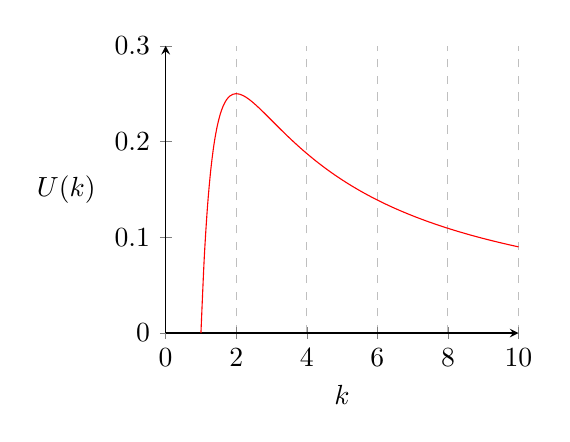
\begin{tikzpicture}
			\begin{axis}[
				axis lines=left, 
				xmin=0,
				xmax=10,
				ymin=0,
				ymax=0.3,
				xlabel=$k$, 
				ylabel=$U(k)$, 
				ylabel style={rotate=-90},
				xmajorgrids,
				grid style={dashed},
				width=0.5\linewidth 
				]
				
				\addplot[
				smooth,
				samples=100, 
				color=red, 
				mark=false,
				domain=1:10
				] {
					(1/x) - (1/(x^2)
				};
			\end{axis}
		\end{tikzpicture}
		\caption{Graph of $U(k) = \frac{1}{k} - \frac{1}{k^{2}}$ for $k \in \mathbb{R}$, $k \neq 0$}
		\label{fig:fourier_uncertainty_function}
	\end{figure}
	\begin{align*}
		\text{setting} \quad \primed{U}(k) & = \dervb{k}{\frac{1}{k} - \frac{1}{k^{2}}} = -\frac{1}{k^{2}} + \frac{2}{k^{3}} = 0 \quad \text{gives critical point } k = 2 \\
		U^{\prime \prime}(k) & = \frac{2}{k^{3}} - \frac{6}{k^{4}} \implies U^{\prime \prime}(2) = -\frac{1}{8} \leq 0 \quad \text{(maxima)}
	\end{align*}
	Hence, $U(k)$ attains maximum value at $k=2$, $max(U(k)) = U(2) = \frac{1}{4}$ (fig \ref{fig:fourier_uncertainty_function}). Finally
	\begin{flalign}\label{eq:fourier_uncertainty_principle}
		\text{\textbf{Fourier Uncertainty Principle}:} \quad \boxed{\variance{t} \variance{\omega} \geq \frac{1}{4} \quad \text{or} \quad \stdev{t} \stdev{\omega} \geq \frac{1}{2}}&&
	\end{flalign}
	
	\section{Towards Quantum World}
	Fourier trade off [eq \eqrefnp{eq:fourier_uncertainty_principle}] gives a \textit{natural} lower bound to the total spread (or uncertainty) in signal and it's spectrum. \quotedsingleit{Natural} signifies it is not a consequence of imperfect measurements, but rather it's a spread fundamental to what a signal even is (spread over time). 
	
	There is nothing special about time here. With carefully crafted relativistic intuition and some quantum principles, this idea can be extended way beyond time to waves spread over space! \cite{de_broglie_thesis}. To understand how a particle can be regarded as wave, we have to consider energy, and how it is carried over space, the idea to which is encapsulated in principles listed below
	\begin{enumerate}
		\item \textbf{Inertia of energy}: Following Einstein, energy is equivalent to mass, and mass represents energy. They are always proportional to each other by
		%	Hence, every energy can be associated with proper mass $m_{0}$ (mass as measured by an observer at rest relative to the body) and vice versa
		\begin{equation*}
			Energy = mass \times c^{2}
		\end{equation*}
		where $c$ is the speed of light, which according to de Broglie is more precisely \quotedsingleit{Limit speed of energy}.
		\item \textbf{Quantum Relation}: Following the description of a Quantum Mechanics, the basic idea behind quanta is that an isolated packet of energy is meaningless without a frequency associated with it
		\begin{equation*}
			Energy = h \times frequency
		\end{equation*}
		where h is plank's constant
	\end{enumerate}
	Following these principles, one can associate each portion of energy with a proper mass $m_{0}$ (mass as measured by an observer at rest relative to the body), as well as with a periodic phenomenon with frequency $\nu_{0}$ 
	\begin{equation*}
		E_{0} = m_{0}c^{2} = h \nu_{0}
	\end{equation*}
	where $m_{0}$ and $\nu_{0}$ are measured in the rest frame of the energy packet.
	
	So if mass is the same as energy, and that energy is carried by some periodic phenomenon, then a particle can be considered as a little wave packet dispersed over space, energy of which is carried in some form of oscillations. Photons show this behavior, as proven by Einstein in Photoelectric effect. De Broglie hypothesis extend this idea to all particles, which can be made clear by a simple analogy.
	\subsection{Mechanical analogy of Wave Nature} \label{sec:mechanical_analogy_to_wave_nature}
	Following is a modified version of the analogy de Broglie had originally proposed \cite{de_broglie_thesis}. Consider a rigid horizontal wire from which identical weights are suspended using springs, such that density of such weights (number of weights per unit length) decreases rapidly as one moves out from the mid point of wire i.e weights are highly concentrated at the center of the wire. Imagine that all weights are oscillating up and down with same frequency, phase and amplitude i.e they are in perfect sync. A virtual thread passing through the center of mass of the weights would then be a straight line, oscillating up and down with same frequency as any of the weight. This ensemble of suspended weights is \quotedsingleit{analogous to a energy packet}, where energy is carried in the oscillations of the virtual thread (Figure \ref{fig:mehanical_analouge_of_wave_rest}).
	\begin{figure}
		\centering
		\subfloat[At rest ($v=0$), all weights are osciallting up and down with same phase.]{
			\label{fig:mehanical_analouge_of_wave_rest}
			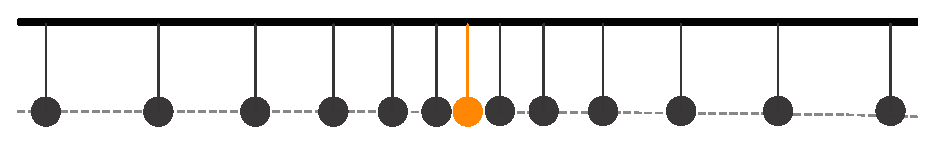
\includegraphics[width=0.96\linewidth]{res/graphics/mechanical_analouge_of_wave_rest.pdf}
		}
		
		\subfloat[At low speeds (ex $v=0.2c$), weights are osciallting with different pahses (dephased)]{
			\label{fig:mehanical_analouge_of_wave_low_speed}
			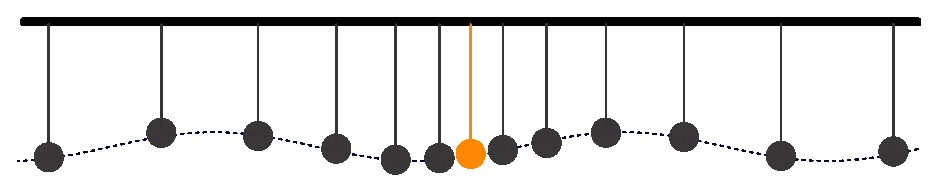
\includegraphics[width=0.96\linewidth]{res/graphics/mechanical_analouge_of_wave_low_speed.pdf}
		}
		
		\subfloat[At high speeds (ex $v=0.6c$), dephasing in the oscillation of weights is highly pronounced]{
			\label{fig:mehanical_analouge_of_wave_high_speed}
			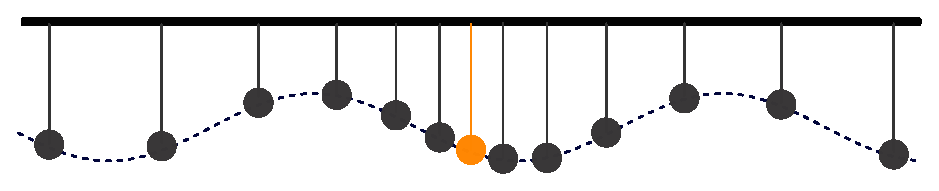
\includegraphics[width=0.96\linewidth]{res/graphics/mechanical_analouge_of_wave_high_speed.pdf}
		}
		
		\caption{Mechanical analogue of a particle dispersed over space as observed in different frames of reference. Dashed line joining the centers of suspended weights is the \quotedsingleit{virtual thread}}
		\label{fig:mehanical_analouge_of_wave}
	\end{figure}
	\begin{flalign}\label{eq:proper_freq_to_rest_energy}
		\text{Proper frequency of oscillation of weights/thread:} \quad \nu_{0} = \frac{m_{0}c^{2}}{h}&&
	\end{flalign}
	
	Up till now, the description is for an observer at rest relative to the system. However, if an observer is moving relative to this system with a uniform velocity $v = \beta c$, then each weight to him would be like a clock, showing Einstein \textbf{\textit{time dilation}}. Also, distribution of weights along the length of wire would no longer be isotropic about the center due to \textbf{\textit{Lorentz or length contraction}}. As a consequence, weights will fall out of phase (Figure \ref{fig:mehanical_analouge_of_wave_low_speed}), and their oscillations appear to slow down by a factor of $\sqrt{1 - \beta^{2}}$ from their proper frequency. An observer in motion relative to the system will then measure the frequency of oscillations as
	\begin{equation}\label{eq:relaativistic_oscillation_freq}
		\nu_{1} = \nu_{0}\sqrt{1 - \beta^{2}} = \frac{m_{0}c^{2}}{h}\sqrt{1 - \beta^{2}}
	\end{equation}
	
	From this moving viewpoint, the virtual thread connecting center of mass of weights will a sinusoid, parallel to the motion of the system. Faster the motion of system relative to observer, higher will be the effects of time dilation and length contraction causing dephasing of weights to be more pronounced, resulting in higher frequency of the sinusoidal virtual thread (Figure \ref{fig:mehanical_analouge_of_wave_high_speed}). Hence, the frequency of sinusoidal thread can be imagined to be associated with the kinetic energy of the system.
	
	From relativistic dynamics, if a body with proper mass $m_{0}$ is in uniform motion with velocity $v = \beta c$ relative to an observer, then it's mass (and consequently energy) as measured by the observer would be
	
	\begin{equation}\label{eq:relativistic_mass_and_energy}
		m_{relativistic} = \frac{m_{0}}{\sqrt{1 - \beta^{2}}} \implies E_{relativistic} = m_{relativistic} \times c^{2} = \frac{m_{0}c^{2}}{\sqrt{1 - \beta^{2}}}
	\end{equation}
	where $\gamma = 1/\sqrt{1 - \beta^{2}}$ is the \textbf{\textit{Lorentz Factor}}. 
	Since kinetic energy is the same as energy gained by a body when brought from rest to velocity $v=\beta c$
	\begin{equation}\label{eq:relativistic_kinetic_energy}
		E_{kinetic} = E_{relativistic} - E_{0} = m_{0}c^{2} \left(\frac{1}{\sqrt{1 - \beta^{2}}} - 1 \right)
	\end{equation}
	which for small $\beta$ reduces to classical form $E_{kinetic} = m_{0}v^{2}/2$.\\ 
	If we associate kinetic energy with the frequency of sinusoidal virtual thread, then
	\begin{equation}\label{eq:relativistic_sinusoidal_virtual_thread_freq}
		\nu = \frac{E_{kinetic}}{h} = \frac{m_{0}c^{2}}{h} \left(\frac{1}{\sqrt{1 - \beta^{2}}} - 1\right)
	\end{equation}
	Notice that the sinusoidal frequency \eqref{eq:relativistic_sinusoidal_virtual_thread_freq} is fundamentally different from oscillation frequency $\nu_{1}$ \eqref{eq:relaativistic_oscillation_freq}, in the way Lorentz factor combines with proper frequency $\nu_{0}=\frac{m_{0}c^{2}}{h}$.
	%as they have different multipliers with proper frequency $\nu_{0}=\frac{m_{0}c^{2}}{h}$
	
	\subsection{The Energy Momentum Relation}
	Lorentz Factor $\gamma = 1/\sqrt{1 - \beta^{2}}$ is  the key to relativistic dynamics. It can also be expressed in terms of momentum $p$, a classical property describing how a body moves through space. \cite{forshaw2014relativity}
	\begin{equation}\label{eq:lorentz_factor_as_func_of_velocity}
		\gamma(v) = \frac{1}{\sqrt{1 - \frac{v^{2}}{c^{2}}}}
	\end{equation}
	\begin{align}
		& p = m_{relativistic} \times v = \frac{m_{0}v}{\sqrt{1 - \beta^{2}}} = \frac{m_{0}v}{\sqrt{1 - \frac{v^{2}}{c^{2}}}} \nonumber \tag{using \eqrefnp{eq:relativistic_mass_and_energy}} \\
		\text{squaring both sides:} \quad & p^{2}\left(1 - \frac{v^{2}}{c^{2}} \right) = m_{0}^{2}v^{2} \nonumber \\
		\text{solving for $v^{2}$:} \quad & p^{2} = v^{2} \left(m_{0}^{2} + \frac{p^{2}}{c^{2}}\right) \implies v^{2} = \frac{p^{2}}{m_{0}^{2} + \frac{p^{2}}{c^{2}}} \label{eq:relativistic_momentum_velocity_relation}
	\end{align}
	using $v^{2}$ from \eqref{eq:relativistic_momentum_velocity_relation} in Lorentz factor \eqref{eq:lorentz_factor_as_func_of_velocity} gives
	\begin{align}
		& \gamma^{2}(v) = \frac{1}{1 - \cfrac{v^{2}}{c^{2}}} = \frac{1}{1 - \cfrac{p^{2}}{m_{0}^{2}c^{2} + p^{2}}} = 1 + \frac{p^{2}}{m_{0}^{2}c^{2}} \nonumber  \\
		& \boxed{\gamma(p) = \sqrt{1 + \frac{p^{2}}{m_{0}^{2}c^{2}}}} \quad \text{where} \quad \gamma(p) \equiv \gamma(m_{rel}v) \equiv \gamma \label{eq:lorentz_factor_as_func_of_momentum}
	\end{align}
	using eq \eqref{eq:lorentz_factor_as_func_of_momentum} in relativistic mass \eqref{eq:relativistic_mass_and_energy}
	\begin{align}
		& m_{relativistic} = m_{0} \gamma = \sqrt{m_{0}^{2} + \frac{p^{2}}{c^{2}}} \nonumber \\
		& E_{relativistic} = m_{relativistic} \times c^{2}\nonumber \\
		& \boxed{E_{relativistic} = \sqrt{m_{0}^{2}c^{4} + p^{2}c^{2}}} \label{eq:energy_momentum_relation}
	\end{align}
	eq \eqref{eq:energy_momentum_relation} is the Energy Momentum Relation for a free particle in flat spacetime. First term is rest energy (invariant), while second term is Kinetic energy (due to relative motion through space). If $p$ is very small, this reduces to the classical form
	\begin{equation*}
		E_{relativistic} \approx m_{0}c^{2} + \frac{p^{2}}{2m_{0}}
	\end{equation*}
	Special cases are
	\begin{enumerate}
		\item \textbf{At Rest}: If particle is at rest relative to the observer, than $p=0$ and \eqref{eq:energy_momentum_relation} simplifies to 
		\begin{equation*}
			E_{0} = m_{0}c^{2} \tag{mass-energy equivalence}
		\end{equation*}
		
		%	\item \textbf{Mass-less Particle}: For particles having very low proper mass $m_{0}$, or $m_{0} = 0$ (mass less particles like photons), relativistic energy is predominantly kinetic
		%	\begin{align}\label{eq:energy_momentum_relation_massless}
			%		E_{relativistic} = pc
			%	\end{align}
		%	One might argue that if $m_{0}=0$ (as for photons), then momentum should be $0$ as well. However, \textit{momentum is a relativistic concept} that describes motion relative to an observer. Photons does indeed have no rest mass, but they can still have relativistic mass. Using principle of inertia of energy in eq \eqref{eq:energy_momentum_relation_massless}
		%	\begin{equation}\label{eq:relativistic_mass_as_p_by_c}
			%		E_{relativistic} = m_{relativistic} \times c^{2} = pc \implies \boxed{m_{relativistic} = \frac{p}{c}}
			%	\end{equation}
		%	which means that \textit{relativistic mass of a massless particle is proportional to its momentum}. This agrees with the fact that massless particles experience gravitational fields. Since a conservation law has to use a tensor, a precise description requires energy-momentum four vector tensor, which is valid for both massive and mass-less particles.
		
		\item \textbf{Massless Particle}: Particles having no proper or rest mass ($m_{0} = 0$) like photons composing light are \quotedsingleit{massless}. They always travel at the speed of light $v=c$, so that no observer can ever catch up to them and see \textit{nothing}. For them, rest mass has no meaning since they are never at rest. The relativistic mass would be \cite{forshaw2014relativity}
		\begin{equation*}
			m_{relativistic} = \frac{m_{0}}{\sqrt{1 - \frac{v^{2}}{c^{2}}}} = \frac{0}{0} \tag{using \eqrefnp{eq:relativistic_mass_and_energy}}
		\end{equation*}
		which is indeterminant and can still be non-zero. Using the general energy-momentum relation \eqref{eq:energy_momentum_relation} with $m_{0} = 0$
		\begin{equation}\label{eq:E_equals_pc_massless}
			\boxed{E_{relativistic} = pc} \qquad \text{(all Kinetic)}
		\end{equation}
		From the principle of inertia of energy, $E_{relativistic} = m_{relativistic} \times c^{2}$
		\begin{equation}\label{eq:relativistic_mass_eq_p_by_c}
			m_{relativistic} \times c^{2} = pc \implies \boxed{m_{relativistic} = \frac{p}{c}}
		\end{equation}
		which means that \textit{relativistic mass of a massless particle is purely kinetic and proportional to its momentum}! This agrees with the fact that massless particles experience gravitational fields.
		
		\item \textbf{High Kinetic Energy limit}: For particles with low proper mass $m_{0}$ and moving at very high speeds (accelerated subatomic particles like electrons), kinetic mass gain can be enormous relative to their proper mass. In that case, rest mass (or energy) can be neglected compared to kinetic mass (or energy).
		\begin{equation}\label{eq:E_equals_pc_high_kinetic_energy}
			\boxed{E_{relativistic} \approx pc} \qquad \text{(predominantly Kinetic)}
		\end{equation}
		
		%	\item \textbf{Massless Particle}:	
		%	For particles having very low proper mass $m_{0}$, or $m_{0} = 0$ (mass less particles like photons), relativistic energy is predominantly kinetic
		%	\begin{align}\label{eq:energy_momentum_relation_massless}
			%		E_{relativistic} = pc
			%	\end{align}
		%	One might argue that if $m_{0}=0$ (as for photons), then momentum should be $0$ as well. However, \textit{momentum is a relativistic concept} that describes motion relative to an observer. Photons does indeed have no rest mass, but they can still have relativistic mass. Using principle of inertia of energy in eq \eqref{eq:energy_momentum_relation_massless}
		%	\begin{equation}\label{eq:relativistic_mass_as_p_by_c}
			%		E_{relativistic} = m_{relativistic} \times c^{2} = pc \implies \boxed{m_{relativistic} = \frac{p}{c}}
			%	\end{equation}
		%	which means that \textit{relativistic mass of a massless particle is proportional to its momentum}. This agrees with the fact that massless particles experience gravitational fields. Since a conservation law has to use a tensor, a precise description requires energy-momentum four vector tensor, which is valid for both massive and mass-less particles.
	\end{enumerate}
	
	\subsection{From Time to Space}
	Following the mechanical analogy in section \ref{sec:mechanical_analogy_to_wave_nature}, if we associate frequency of sinusoidal virtual thread with the kinetic energy from energy-momentum relation (eq \eqrefnp{eq:energy_momentum_relation}, \eqrefnp{eq:E_equals_pc_massless} and \eqrefnp{eq:E_equals_pc_high_kinetic_energy})
	\begin{equation*}
		\nu = \frac{E}{h} = \frac{pc}{h}
	\end{equation*}
	
	Analogous to temporal frequency $\nu = 1/T$ cycles per unit time, where $T$ is the time period (time required for a wave to complete one cycle), \textbf{\textit{spatial frequency}} $\bar{\nu} = 1/ \lambda$ cycles per unit distance, where $\lambda$ is the distance period (distance traveled by wave in one cycle). Using $c=\nu \lambda$
	\begin{equation}\label{eq:momentum_spatial_freq_relation}
		\nu = \frac{c}{\lambda} = c \bar{\nu} = \frac{pc}{h} \implies \boxed{p = h\bar{\nu}}
	\end{equation}
	Equation \eqref{eq:momentum_spatial_freq_relation} has a highly significant message. \textit{The momentum of a particle is proportional to the spatial frequency of the wave describing its motion through space}, the one we have been calling sinusoidal virtual thread!. This is the infamous Louis de Broglie hypothesis, saying that \textit{momentum is the same as spatial frequency}. Following relativistic mass of photons (eq \eqrefnp{eq:relativistic_mass_eq_p_by_c})
	\begin{equation}\label{eq:relativistic_mass_proportional_to_spatial_freq}
		m_{relativistic} = \frac{p}{c} \implies \boxed{m_{relativistic} = \frac{h}{c}\bar{\nu}}
	\end{equation}
	equation \eqref{eq:relativistic_mass_proportional_to_spatial_freq} implies that relativistic mass of a massless particle ($m_{0}=0$) is proportional to the spatial frequency of the wave describing its motion through space.
	
	\subsection{From Fourier to Quantum Uncertainty Principle}
	If $a$ is a continuous random variable with probability distribution $A(a)$,  such that $a = kb$ where $k$ is proportionality constant, $a, b \in \mathbb{R}$, then their variance are related as
	
	\begin{align}
		\variance{a} & = \intinfty (a - \bar{a})^{2} P(a) \diff a = \frac{\intinfty (a - \bar{a})^{2} |A(a)|^{2} \diff a}{\intinfty |A(a)|^{2} \diff a} \nonumber \\
		& = \frac{\intinfty k^{2}(b - \bar{b})^{2} |A(b)|^{2} \diff b}{\intinfty |A(b)|^{2} \diff b} = k^{2} \variance{b} \nonumber \\
		\variance{a} & = k^{2} \variance{b} \implies \boxed{\stdev{a} = k \stdev{b}} \label{eq:variance_of_proportional_quantities}
	\end{align}
	since standard deviation is a measure of spread from the mean, negative root is neglected.
	
	From Fourier uncertainty principle (equation \eqrefnp{eq:fourier_uncertainty_principle})
	\begin{equation}\label{eq:time_temporal_freq_uncertainty_principle}
		\stdev{t} \stdev{\omega} \geq \frac{1}{2} \implies \boxed{\stdev{t} \stdev{\nu} \geq \frac{1}{4\pi}} \qquad \text{(using $\omega = 2\pi \nu$ and eq \eqrefnp{eq:variance_of_proportional_quantities})}
	\end{equation}
	equation \eqref{eq:time_temporal_freq_uncertainty_principle} is the Time-Temporal frequency uncertainty principle. For a particle in uniform motion with velocity $v = x / t$ and associated spatial wave with frequency $\bar{\nu} = \nu / v$, where $\bar{\nu} = 1/\lambda$ is the spatial frequency, eq \eqref{eq:variance_of_proportional_quantities} gives
	%since $v = \nu \lambda \implies v\bar{\nu} = \nu$
	\begin{align}
		& x = vt \implies \stdev{x} = v\stdev{t} \nonumber \\
		& \bar{\nu} = \frac{\nu}{v} \implies \stdev{\bar{\nu}} = \frac{\stdev{\nu}}{v} \nonumber \\
		& \stdev{x}\stdev{\bar{\nu}} = \stdev{t} \stdev{\nu} \implies \boxed{\stdev{x}\stdev{\bar{\nu}} \geq \frac{1}{4\pi}} \quad \text{(using \eqrefnp{eq:time_temporal_freq_uncertainty_principle})} \label{eq:space_spatial_freq_uncertainty_principle}
	\end{align}
	equation \eqref{eq:space_spatial_freq_uncertainty_principle} is the Space-Spatial frequency uncertainty principle for waves spread over space. Using proportionality of momentum and spatial frequency (eq \eqrefnp{eq:momentum_spatial_freq_relation})
	\begin{align}
		& p = h \bar{\nu} \implies \stdev{\bar{\nu}} = \frac{\stdev{p}}{h}  \nonumber \\
		& \stdev{x}\stdev{\bar{\nu}} = \frac{\stdev{x}\stdev{p}}{h} \geq \frac{1}{4 \pi} \nonumber \tag{using \eqrefnp{eq:space_spatial_freq_uncertainty_principle}} \\
		& \boxed{\stdev{x}\stdev{p} \geq \frac{h}{4 \pi}} \label{eq:heisenberg_uncertainty_principle}
	\end{align}
	equation \eqref{eq:heisenberg_uncertainty_principle} is the infamous \textbf{Heisenberg's uncertainty principle}!. It's astonishing how a simple idea of frequency decomposition of a signal can manifest to such huge implications.
	
	\section{Conclusion}
	The lesson from this is that Heisenberg's uncertainty principle is not an artifact of randomness or imperfect measurements in the quantum realm. Rather, it's a fundamental trade-off between how concentrated a wave and it's frequency representation can be, applied in the context of wave nature of the particle (i.e saying particle is a wave and spread out over space). Space and spatial frequency (which is the same as momentum $p=h\bar{\nu}$) share the same trade-off as time and temporal frequency. The trade-off in itself is however quite general and shows up in many real world non-quantum cases as well!
	
	%Origin of these two effects on time and space is due to a core fact from Special Relativity 'Events that appear to be simultaneous from one viewpoint, many not be simultaneous in another reference frame'.
	% Appendix
	\section{Appendix}\label{sec:appendix}
	
	% Fbini's Theorem
	\subsection{Fubini's Theorem}\label{sec:fubini_theorem}
	Multiple integrals can be replaced by iterated integrals (or vice-versa), and the order of integration can be switched, provided multiple integral 
	of the absolute integrand converges. Mathematically
	\begin{flalign*}
		\text{If} \quad \iint \limits _{X\times Y}|f(x,y)| \dx \dy < \infty&&
	\end{flalign*}
	\begin{equation}\label{eq:fubini}
		\text{Then} \quad \iint \limits _{X\times Y}f(x,y) \dx \dy =\int _{X}\left(\int _{Y}f(x,y) \dy \right) \dx =\int _{Y}\left(\int _{X}f(x,y) \dx \right) \dy
	\end{equation}
	
	\subsection{Leibniz integral rule}\label{sec:leibniz_integral_rule}
	Leibniz integral rule of differentiation under the integral sign is
	\begin{equation}\label{eq:leibniz_integral_rule}
		\dervb{x}{\dint{a}{b} f(x,t) \dt} = \dint{a}{b} \pderv{x}f(x,t) \dt
	\end{equation}
	Method that uses this rule to compute integrals is known as \quotedsingleit{Feynman's method}
	
	% Delta Function (P.A.M Dirac (1902-1984) in his book 'The principles of Quantum mechanics, Oxford University press, 1958' originally published in 1930)
	\subsection{Dirac Delta Function}\label{sec:delta_func}
	The Dirac delta function $\delta(x)$ is a generalized distribution over real numbers defined by two key properties \cite{dirac1981qm}
	\begin{equation}\label{eq:delta_func_def}
		\delta (x) = \left\{
		\begin{array}{ll}
			0  &  \quad \text{ if } x \neq 0 \\
			\infty & \quad \text{ if } x = 0
		\end{array}
		\right. \qquad \text{(only turns on at $0$)}
	\end{equation}
	and
	\begin{equation}\label{eq:delta_func_area}
		\intinfty \delta (x) \dx = 1 \qquad \text{(area under distribution is $1$)}
	\end{equation}
	This leads to the following
	\begin{enumerate}
		\item Integration Property
		\begin{flalign}\label{eq:delta_func_integration_value}
			\intinfty f(x)\delta (x-a) \dx v= \intinfty f(a)\delta (x-a) \dx = f(a)\intinfty \delta (x-a) \dx = f(a)&&
		\end{flalign}
		where second integral comes from the fact that $\delta (x - a)$, and consequently the integrand is $0$ everywhere except when $x=a$, so that only $f(x=a)$ contributes to the integral, which is constant and can be moved outside
		\item Another independent definition of delta function, following Appendix \ref{sec:int_complex_exp}
		\begin{flalign}\label{eq:delta_func_def_complex_exp}
			\intinfty e^{i\omega t} \domega = 2\pi \delta (t)&&
		\end{flalign}
	\end{enumerate}
	
	% Integral of sin(x)/x
	\subsection{Definite Integral of sin(x)/x}\label{sec:int_sinx_by_x}
	\begin{equation}\label{eq:int_sinx_by_x}
		\intzerotoinfty \frac{\sin(x)}{x} \dx = \frac{\pi}{2}
	\end{equation}
	
	\vspace{4pt}
	\textbf{Proof}: \cite{herman2016fourieranalysis} This is an improper integral since the integrand $\sin(x) / x$ has $x$ in the denominator, but still converges. In order to actually integrate this, we need a way to somehow eliminate the $x$ in denominator while keeping the integrand convergent. One way to do that is to multiply the integrand with some function of x and a parameter $b$, which when differentiated with respect to $b$ under the integral sign eliminates $x$ (Feynman's Technique, Appendix \ref{sec:leibniz_integral_rule}).
	
	One such function is $e^{bx}$, $b \in \mathbb{R}$. However, this diverges in the limit $x \to \infty$, and can only converge if the exponent is negative. So the best choice is $e^{-bx}$, $b > 0$ which converges in the limit $x \to \infty$. Defining the parameterized integral
	\begin{equation}\label{eq:sinx_by_x_parametrized_integral}
		I(b) = \intzerotoinfty \frac{\sin(x) e^{-bx}}{x} \dx
	\end{equation}
	our goal is to find $I(b=0)$. Differentiating with respect to b
	\begin{align*}
		\primed{I}(b) & = \derv{b}I(b) = \dervb{b}{\intzerotoinfty \frac{\sin(x) e^{-bx}}{x} \dx} \\
		& = \intzerotoinfty \pdervb{b}{\frac{\sin(x) e^{-bx}}{x}} \dx = -\intzerotoinfty \sin(x) e^{-bx} \dx \tag{using \eqrefnp{eq:leibniz_integral_rule}}
	\end{align*}
	integrating by parts, taking $\sin(x)$ as first and $e^{-bx}$ as second function gives
	\begin{equation*}
		\primed{I}(b) = \left[\frac{e^{-bx}}{1 + b^{2}} \left(b\sin(x) + \cos(x)\right)\right]_{x=0}^{x=\infty} = -\frac{1}{1 + b^{2}}
	\end{equation*}
	integrating with respect to b
	\begin{align}
		& \int \primed{I}(b) \diff b = I(b) = -\tan^{-1}(b) + c \nonumber \\
		\implies & I(b=0) = c, \quad I(b=\infty) = -\frac{\pi}{2} + c = -\frac{\pi}{2} + I(b=0) \label{eq:sinx_by_x_parametrized_integral_results}
	\end{align}
	where c is the constant of integration. Since by definition of $I(b)$ (eq \eqrefnp{eq:sinx_by_x_parametrized_integral})
	\begin{align*}
		& I(b) = \intzerotoinfty \frac{\sin(x) e^{-bx}}{x} \dx \implies I(b=\infty) = 0 \\
		\text{So} \quad & I(b=\infty) = 0 = -\frac{\pi}{2} + I(b=0) \tag{using \eqrefnp{eq:sinx_by_x_parametrized_integral_results}} \\
		& \boxed{I(b=0) = \frac{\pi}{2}}
	\end{align*}
	which is the required integral. In general, if $k \in \mathbb{R}, k > 0$, then
	\begin{equation}\label{eq:int_sinkx_by_x}
		\int \limits_{x=0}^{x=\infty} \frac{\sin(kx)}{x} \dx = \int \limits_{y=0}^{y=\infty} \frac{\sin(y)}{y} \dy = \frac{\pi}{2}
	\end{equation}
	where second integral results from substitution $y=kx$
	% Integral of complex exponential
	\subsection{Definite Integral of Complex Exponential}\label{sec:int_complex_exp}
	\begin{equation}\label{eq:int_complex_exp}
		\intinfty e^{i\omega t} \domega = 2\pi \delta (t)
	\end{equation}
	
	\vspace{4pt}
	\textbf{Proof}: \cite{herman2016fourieranalysis} let $I(t) = \intinfty e^{i\omega t} \domega$ be the required integral, and $f_{k}(t), k\in \mathbb{R}, k > 0$ be its a generalized form defined as
	\begin{equation}\label{eq:int_complex_exp_It_as_fkt}
		f_{k}(t) = \dint{-k}{k} e^{i\omega t} \domega \implies I(t) = \lim\limits_{k \to \infty} f_{k}(t)
	\end{equation}
	However, $f_{k}(t)$ can be easily computed as
	\begin{equation}\label{eq:int_complex_exp_fkt}
		f_{k}(t) = \dint{-k}{k} e^{i\omega t} \domega = \left[\frac{e^{i\omega t}}{it}\right]_{\omega=-k}^{\omega=k} = \frac{e^{ikt} - e^{-ikt}}{it} = \frac{2\sin(kt)}{t}
	\end{equation}
	where $e^{ikt}=\cos(kt) + i\sin(kt)$ is the Euler's formula. Equation \eqref{eq:int_complex_exp_fkt} shows that $f_{k}(t)$ is an \textit{even function} (as $k > 0$) containing the improper integrand $\sin(kt)/t$ (section \ref{sec:int_sinx_by_x})
	\begin{align}
		\intinfty f_{k}(t) \dt & = \intinfty \frac{2\sin(kt)}{t} \dt = 4 \intzerotoinfty \frac{\sin(kt)}{t} \dt = 2\pi	\tag{using \eqrefnp{eq:int_sinkx_by_x}} \nonumber \\
		\text{divide by $2\pi$:} \quad & \intinfty \frac{f_{k}(t)}{2\pi} \dt = \intinfty \frac{\sin(kt)}{\pi t} \dt = 1 \label{eq:int_complex_exp_area_under_fkt_1}
	\end{align}
	equation \eqref{eq:int_complex_exp_area_under_fkt_1} looks similar to the area property of delta function (eq \eqrefnp{eq:delta_func_area}). The graph of the integrand $\sin(kt)/\pi t$ (figure \ref{fig:sin_kx_by_pix}) suggests that at high $k$ values, it is essentially $0$ everywhere except a huge peak at $t=0$. In the limit of $k \to \infty$
	\begin{figure}
		\centering
		\subfloat[$k = 10$] {
			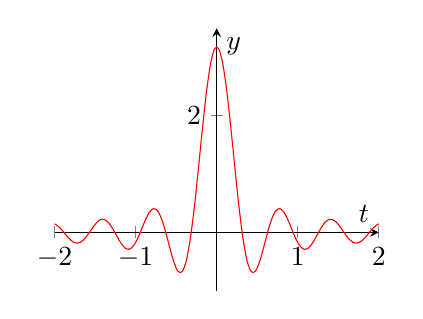
\begin{tikzpicture}
				\label{fig:sin_kx_by_pix_low_k}
				\begin{axis} [
					axis lines=middle, 
					xmin=-2, 
					xmax=2, 
					ymin=-1,
					ymax=3.5,
					xlabel=$t$, 
					ylabel=$y$, 
					ylabel style={rotate=0}, 
					width=0.47\linewidth
					]
					
					\addplot[
					smooth,
					color=red, 
					samples=200,
					mark=false
					] {
						sin(deg(10 * x)) / (pi * x)
					};
					
				\end{axis}
			\end{tikzpicture}
		}\hfill
		\subfloat[$k = 100$] {
			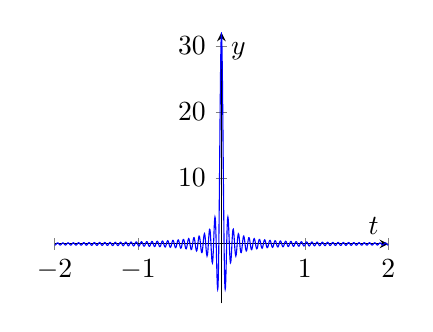
\begin{tikzpicture}
				\label{fig:sin_kx_by_pix_high_k}
				%			\begin{axis} [     % k=50
					%				axis lines=middle, 
					%				xmin=-2, 
					%				xmax=2, 
					%				ymin=-3,
					%				ymax=16,
					%				xlabel=$t$, 
					%				ylabel=$y$, 
					%				ylabel style={rotate=0}, 
					%				width=0.45\linewidth
					%				]
					%				
					%				\addplot[
					%				smooth,
					%				color=blue, 
					%				samples=200,
					%				mark=false
					%				] {
						%					sin(deg(50 * x)) / (pi * x)
						%				};
					%				
					%			\end{axis}
				\begin{axis} [
					axis lines=middle, 
					xmin=-2, 
					xmax=2, 
					ymin=-9,
					ymax=32,
					xlabel=$t$, 
					ylabel=$y$, 
					ylabel style={rotate=0}, 
					width=0.48\linewidth
					]
					
					\addplot[
					smooth,
					color=blue, 
					samples=2000,
					mark=false
					] {
						sin(deg(100 * x)) / (pi * x)
					};
					
				\end{axis}
			\end{tikzpicture}
		}
		
		\caption{Plot of $\sin(kt)/\pi t$ against $t$ for different $k > 0, k \in \mathbb{R}$. As $k$ increases, function approaches $k/\pi$ for $t = 0$ and tends to $0$ for $t \neq 0$}
		\label{fig:sin_kx_by_pix}
	\end{figure}
	
	\begin{equation}\label{eq:int_complex_exp_delta_analouge_switching}
		\lim \limits_{k \to \infty} \frac{\sin(kt)}{\pi t} = \left\{
		\begin{array}{ll}
			0  &  \quad \text{ if } t \neq 0 \\
			\infty & \quad \text{ if } t = 0
		\end{array}
		\right.
	\end{equation}
	from the two properties of $\sin(kt)/\pi t$ in equation \eqref{eq:int_complex_exp_delta_analouge_switching} and \eqref{eq:int_complex_exp_area_under_fkt_1}, it is clear that
	\begin{equation*}
		\lim \limits_{k \to \infty} \frac{\sin(kt)}{\pi t} = \delta(t)
	\end{equation*}
	Using the definitions of $f_{k}(t)$ from equation \eqref{eq:int_complex_exp_It_as_fkt} and \eqref{eq:int_complex_exp_fkt}
	\begin{align*}
		& \frac{\sin(kt)}{\pi t} = \frac{f_{k}(t)}{2\pi} \implies \lim \limits_{k \to \infty} \frac{\sin(kt)}{\pi t} = \lim \limits_{k \to \infty} \frac{f_{k}(t)}{2\pi} = \delta(t) \\
		& \lim \limits_{k \to \infty} f_{k}(t) = 2 \pi \delta(t) \implies \boxed{I(t) = 2 \pi \delta(t)}
	\end{align*}
	
	\bibliography{references}
	
	%\subsection{Time dilation and Length Contraction}
	%\subsubsection{Time Dilation (or Clock Retardation)}
\end{document}